\documentclass[11pt]{article}

\usepackage[margin=1in]{geometry}
\usepackage[T1]{fontenc}
\usepackage[utf8]{inputenc}
\usepackage{lmodern}
\usepackage{microtype}
\usepackage{graphicx}
\usepackage{xcolor}
\usepackage{booktabs}
\usepackage{longtable}
\usepackage{array}
\usepackage{enumitem}
\usepackage{hyperref}
\usepackage{tikz}
\usepackage{listings}
\usetikzlibrary{arrows.meta, positioning, shapes.geometric, fit}

\hypersetup{
  colorlinks=true,
  linkcolor=blue!55!black,
  urlcolor=blue!55!black,
  citecolor=blue!55!black
}

\definecolor{recceblue}{HTML}{0EA5E9}
\definecolor{reccedark}{HTML}{0F172A}
\definecolor{reccegreen}{HTML}{10B981}
\definecolor{reccegray}{HTML}{64748B}

\lstdefinestyle{reccecode}{
  basicstyle=\ttfamily\small,
  breaklines=true,
  frame=single,
  framerule=0.3pt,
  rulecolor=\color{reccegray},
  columns=fullflexible,
  keepspaces=true,
  showstringspaces=false,
  backgroundcolor=\color{black!2}
}
\lstset{style=reccecode}

\title{\textbf{Recce: An End-to-End Automation Platform for AI-Assisted Film Location Scouting}}
\author{Arun Sharma}
\date{June 2026}

\begin{document}
\maketitle

\begin{abstract}
Recce is a deployable film-location scouting system that converts screenplay
material into structured location briefs, visually ranked real-world candidates,
route plans, mood-board references, and shoot-day logistics packets. The system
combines language-model scene understanding, server-side map and imagery
services, deterministic fallback modules, open location and permit data, route
optimization, sun-window computation, weather summaries, and a production-facing
React workspace. This white paper documents the current architecture, execution
model, test strategy, and Kubernetes deployment path. It is written as both a
technical reference and a starter guide for running, testing, and scaling Recce.
\end{abstract}

\section{Executive Summary}

Film location scouting is a high-context workflow. A location manager must read
scene intent, infer production constraints, search for real places, judge visual
fit, understand permit and access requirements, plan a scout route, and produce
usable notes for the production team. Recce compresses that workflow into a
single tool surface. The application accepts a scene or full script, extracts
one or more location briefs, produces candidate locations, scores those
candidates against the director's brief, supports shortlist selection on a map,
optimizes a scout day, and generates a logistics packet.

\paragraph{Core contribution:}
Recce moves beyond keyword search. It treats each candidate as an operational
scouting decision: does the real place visually fit the scene, can it be reached
efficiently, what permits or restrictions are implied, what sun and weather
conditions matter, and what starter shot list supports the scene?

\paragraph{Current implementation:}
The repository contains a FastAPI backend and a Vite/React frontend served by a
single production container. Demo mode works without API keys through bundled
briefs and candidates, deterministic script segmentation, demo weather, and
placeholder concept frames. Live mode can be enabled through Gemini, Google
Maps, OSRM, weather providers, and normalized permit datasets.

\section{Application Screenshot}

Figure~\ref{fig:app-screenshot} shows the current production-facing workspace:
script input and filters on the left, map in the center, and the generated
shoot-day packet on the right.

\begin{figure}[ht]
  \centering
  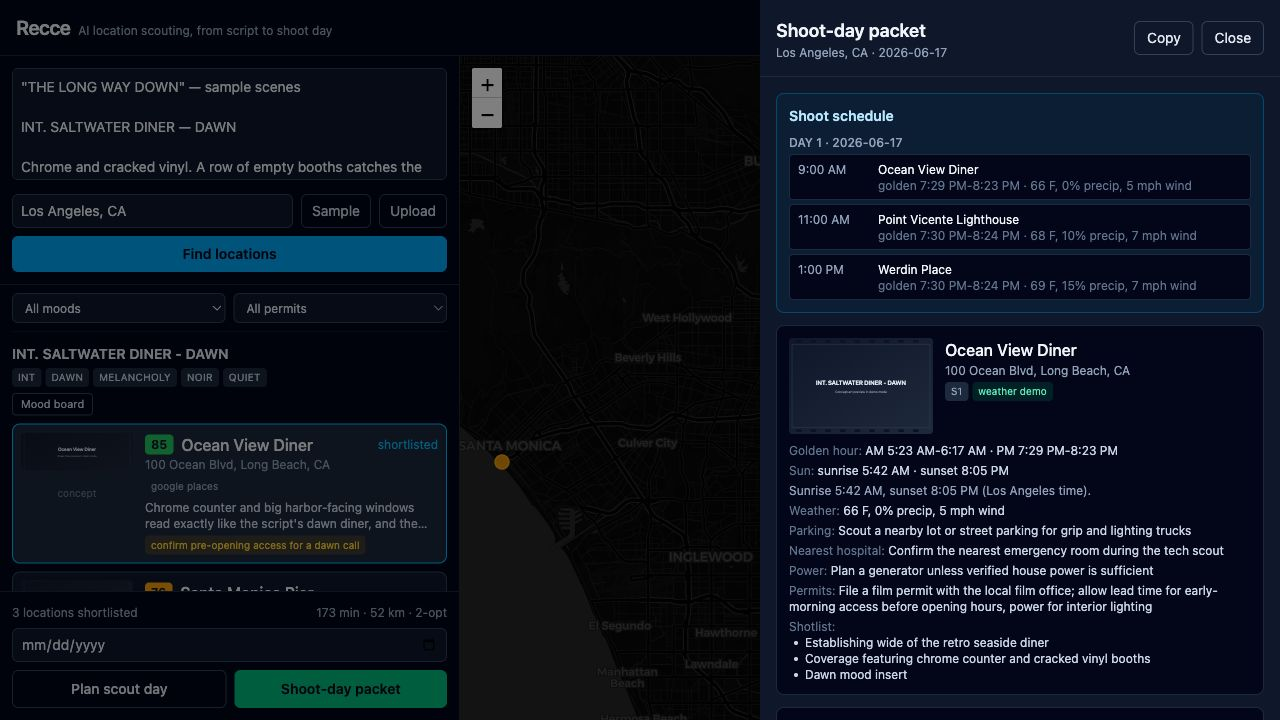
\includegraphics[width=\linewidth]{assets/recce-packet-workflow.png}
  \caption{Recce demo workflow after loading the bundled sample, finding candidates,
  planning a route, and opening the shoot-day packet.}
  \label{fig:app-screenshot}
\end{figure}

\section{System Goals}

\paragraph{Production usefulness:}
The output must be usable by location managers, line producers, and directors.
That means the system cannot stop at a ranked search list. It must expose
constraints such as access, permit risk, weather, sun windows, driving time, and
crew logistics.

\paragraph{Demo reliability:}
The full workflow must run without API keys. This is important for review,
education, hackathon demos, and early design-partner evaluation. Demo mode
therefore uses bundled data, deterministic fallbacks, and placeholder images.

\paragraph{Live-mode extensibility:}
The same code path must support real service providers when keys and URLs are
configured. Candidate search, image scoring, routing, weather, and mood-board
generation are encapsulated so each live provider can be switched on
independently.

\paragraph{Scalable deployment:}
The production artifact is a single HTTP service. Kubernetes deployment adds
replicas, health probes, autoscaling, disruption protection, network policy, and
non-root execution.

\section{End-to-End Workflow}

\begin{figure}[ht]
\centering
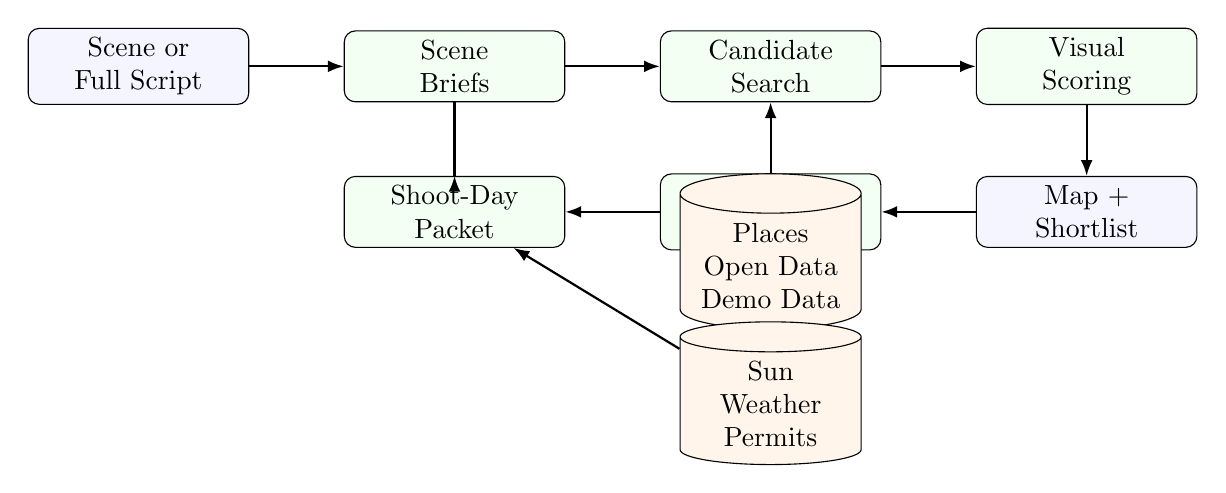
\begin{tikzpicture}[
  node distance=0.9cm and 1.2cm,
  box/.style={draw, rounded corners, align=center, minimum width=2.8cm, minimum height=0.9cm, fill=blue!4},
  service/.style={draw, rounded corners, align=center, minimum width=2.8cm, minimum height=0.9cm, fill=green!5},
  data/.style={draw, cylinder, shape border rotate=90, aspect=0.25, align=center, minimum width=2.3cm, minimum height=0.9cm, fill=orange!8},
  arrow/.style={-{Latex[length=2mm]}, thick}
]
\node[box] (script) {Scene or\\Full Script};
\node[service, right=of script] (briefs) {Scene\\Briefs};
\node[service, right=of briefs] (cands) {Candidate\\Search};
\node[service, right=of cands] (score) {Visual\\Scoring};
\node[box, below=of score] (ui) {Map +\\Shortlist};
\node[service, left=of ui] (route) {Route\\Optimizer};
\node[service, left=of route] (packet) {Shoot-Day\\Packet};
\node[data, below=of cands] (data) {Places\\Open Data\\Demo Data};
\node[data, below=of route] (env) {Sun\\Weather\\Permits};

\draw[arrow] (script) -- (briefs);
\draw[arrow] (briefs) -- (cands);
\draw[arrow] (cands) -- (score);
\draw[arrow] (score) -- (ui);
\draw[arrow] (ui) -- (route);
\draw[arrow] (route) -- (packet);
\draw[arrow] (data) -- (cands);
\draw[arrow] (env) -- (packet);
\draw[arrow] (briefs.south) |- (packet.north);
\end{tikzpicture}
\caption{High-level Recce workflow from screenplay input to shoot-day packet.}
\label{fig:workflow}
\end{figure}

\paragraph{Scene analysis:}
The backend receives raw screenplay text through \texttt{/api/analyze}. In live
mode, Gemini extracts structured \texttt{SceneBrief} objects. In demo or
fallback mode, \texttt{script\_analysis.py} segments screenplay sluglines and
derives location type, time of day, character cues, mood hints, visual keywords,
practical needs, and search queries.

\paragraph{Candidate generation:}
\texttt{places.py} calls Google Places when a Maps key is configured. Without a
key, it serves bundled candidates. \texttt{permits.py} enriches candidates with
normalized open-data location records, permit flags, permit contacts, and
restrictions. This allows the UI to filter by permit risk even in demo mode.

\paragraph{Visual scoring:}
When Gemini and Maps are both configured, the system fetches the candidate's
best available image, preferring venue photography over Street View, and asks
Gemini to score the image against the director's brief. In demo mode, candidate
scores and rationales come from bundled data plus open-data priors.

\paragraph{Route planning:}
\texttt{routing.py} uses OSRM Trip routing when \texttt{RECCE\_OSRM\_URL} is
configured. If OSRM is unavailable, the system falls back to a deterministic
nearest-neighbor seed followed by 2-opt improvement over haversine distances.

\paragraph{Packet generation:}
\texttt{packet.py} combines shortlisted candidates, briefs, sun windows from
\texttt{astral}, weather summaries, permit metadata, concept-frame URLs, and
Gemini or canned production notes. The packet includes a multi-day schedule
that rolls over after four locations per day.

\section{Backend Architecture}

\begin{longtable}{>{\raggedright\arraybackslash}p{0.24\linewidth} >{\raggedright\arraybackslash}p{0.68\linewidth}}
\toprule
\textbf{Module} & \textbf{Responsibility} \\
\midrule
\endhead
\texttt{routes.py} & FastAPI route surface for health, demo scene, analysis, segmentation, candidates, route, packet, image proxying, and moodboard generation. \\
\texttt{schemas.py} & Pydantic models for briefs, scenes, candidates, route results, packets, weather summaries, schedule stops, and request bodies. \\
\texttt{gemini.py} & Live Gemini integration for scene extraction, visual scoring, location notes, and image generation provider calls. \\
\texttt{script\_analysis.py} & Deterministic screenplay segmentation and fallback brief generation. \\
\texttt{places.py} & Google Places, Street View, Place Photos, geocoding, demo candidates, and safe SVG placeholders. \\
\texttt{permits.py} & Open-data location records, permit enrichment, source metadata, restrictions, and candidate merge logic. \\
\texttt{moodboard.py} & Prompt construction, live image-byte generation, packet-safe data URLs, and placeholder concept-frame URLs. \\
\texttt{routing.py} & Route result construction, OSRM handoff, haversine distance, nearest-neighbor seed, and 2-opt fallback. \\
\texttt{osrm.py} & Optional OSRM Table and Trip HTTP client. \\
\texttt{astro.py} & Time-zone approximation and golden-hour, sunrise, and sunset calculations. \\
\texttt{weather.py} & Demo, Open-Meteo, and OpenWeather forecast summaries. \\
\texttt{packet.py} & Final packet assembly, permit-note merging, weather injection, concept image URLs, and schedule construction. \\
\bottomrule
\end{longtable}

\section{Frontend Architecture}

The frontend is a Vite/React/TypeScript application with a dense scouting
workspace. It intentionally avoids a marketing-style landing page because the
target user needs a working operational tool. The first viewport contains script
input, base city, upload controls, scene filters, candidate cards, map state,
route controls, and packet generation.

\paragraph{Core views:}
\begin{itemize}[leftmargin=*]
  \item \textbf{Script intake:} Paste screenplay text, load the sample, or upload
  a text-like script file.
  \item \textbf{Scene selection:} Full scripts can be segmented into scene
  checkboxes before candidate search.
  \item \textbf{Candidate review:} Candidate cards show real imagery, concept
  placeholders, match scores, source labels, permit badges, rationales, and
  flags.
  \item \textbf{Map view:} Leaflet renders selected candidates and route context
  with keyless OpenStreetMap tiles.
  \item \textbf{Packet drawer:} The generated packet shows schedule, concept
  frames, sun windows, weather, parking, power, permit notes, restrictions, and
  starter shot lists.
\end{itemize}

\section{API Surface}

\begin{longtable}{>{\raggedright\arraybackslash}p{0.22\linewidth} >{\raggedright\arraybackslash}p{0.16\linewidth} >{\raggedright\arraybackslash}p{0.54\linewidth}}
\toprule
\textbf{Endpoint} & \textbf{Method} & \textbf{Purpose} \\
\midrule
\endhead
\texttt{/api/health} & GET & Returns status, demo mode, key availability booleans, OSRM availability, model name, and weather provider. \\
\texttt{/api/demo/scene} & GET & Returns the bundled sample screenplay. \\
\texttt{/api/script/segments} & POST & Segments a full script into deterministic scene records. \\
\texttt{/api/analyze} & POST & Produces structured scene briefs from screenplay text. \\
\texttt{/api/candidates} & POST & Produces candidate locations for one or more briefs. \\
\texttt{/api/route} & POST & Optimizes a scout-day route over shortlisted candidates. \\
\texttt{/api/packet} & POST & Builds the shoot-day logistics packet. \\
\texttt{/api/streetview} & GET & Proxies Street View or returns a safe placeholder image. \\
\texttt{/api/placephoto} & GET & Proxies a Places photo or returns a safe placeholder image. \\
\texttt{/api/moodboard} & POST & Generates or placeholders a scene concept frame. \\
\bottomrule
\end{longtable}

\section{Data Contracts}

The core models are intentionally small and typed. A \texttt{SceneBrief}
contains the scouting requirements inferred from the script. A \texttt{Candidate}
contains a real or demo location, visual score, imagery URL, permit flags, and
source metadata. A \texttt{RouteResult} contains ordered \texttt{RouteStop}
objects plus distance, duration, and route method. A \texttt{Packet} contains
locations, schedule days, production title, date, base city, notes, weather, sun
windows, permits, and shot lists.

\paragraph{Backward compatibility:}
New model fields use defaults. Existing demo JSON and older clients continue to
parse because added fields are optional or defaulted in Pydantic.

\section{Testing Strategy}

The repository implements eight practical test categories. All backend tests run
in demo mode by default through \texttt{backend/tests/conftest.py}. This prevents
local API keys from changing CI behavior.

\begin{longtable}{>{\raggedright\arraybackslash}p{0.18\linewidth} >{\raggedright\arraybackslash}p{0.58\linewidth} >{\raggedright\arraybackslash}p{0.16\linewidth}}
\toprule
\textbf{Type} & \textbf{Coverage} & \textbf{Command} \\
\midrule
\endhead
Unit & Script parsing, permit enrichment, routing, weather, sun math, mood prompts, image placeholders. & \texttt{make test-unit} \\
Integration & API route interactions, response parsing, mocked OSRM and Open-Meteo behavior. & \texttt{make test-integration} \\
End-to-end & Full script-to-packet workflow through the API. & \texttt{make test-e2e} \\
Smoke & Fast health and minimum viable workflow checks. & \texttt{make test-smoke} \\
Contract & OpenAPI endpoints, Pydantic response models, Kubernetes object contracts. & \texttt{make test-contract} \\
Regression & Demo-scene stability and packet schedule rollover behavior. & \texttt{make test-regression} \\
Performance & Local demo pipeline and route optimizer runtime budgets. & \texttt{make test-performance} \\
Security/config & Secret hygiene, placeholder escaping, non-root Kubernetes settings, network policy. & \texttt{make test-security} \\
\bottomrule
\end{longtable}

\paragraph{Smoke runner:}
A no-dependency Python script can validate a running service locally, in
Kubernetes, or on Cloud Run:

\begin{lstlisting}
python3 scripts/smoke_api.py --base-url http://127.0.0.1:8000
python3 scripts/smoke_api.py --base-url https://recce-216756172879.us-central1.run.app
\end{lstlisting}

\paragraph{Frontend checks:}
The frontend target runs TypeScript build, a static UI/API surface smoke check,
and ESLint:

\begin{lstlisting}
make test-frontend
\end{lstlisting}

\section{Kubernetes Deployment Architecture}

The Kubernetes base under \texttt{k8s/base} uses Kustomize and includes a
namespace, config map, optional secret reference, deployment, service,
horizontal pod autoscaler, pod disruption budget, network policy, and ingress.

\begin{figure}[ht]
\centering
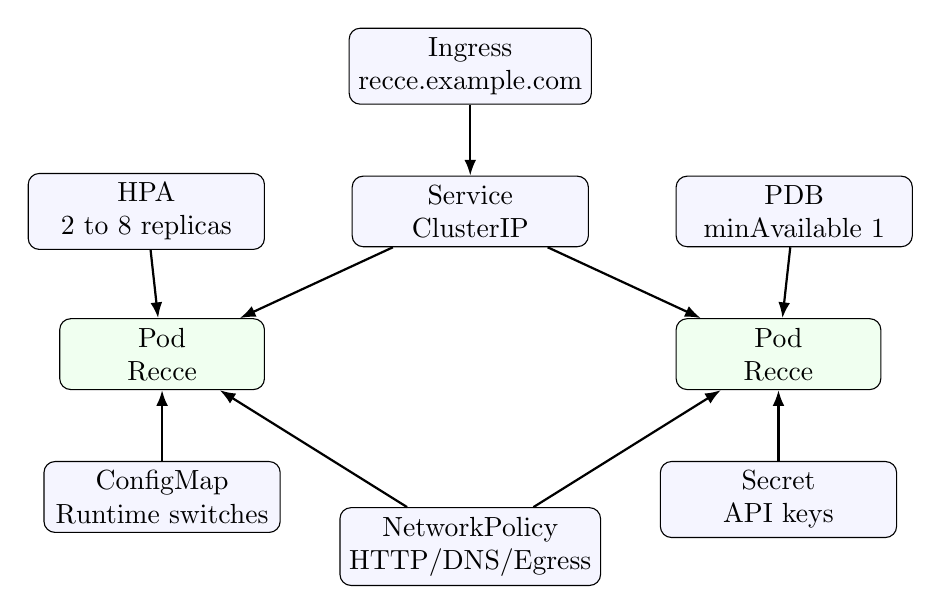
\begin{tikzpicture}[
  node distance=0.9cm and 1.1cm,
  box/.style={draw, rounded corners, align=center, minimum width=3.0cm, minimum height=0.85cm, fill=blue!4},
  pod/.style={draw, rounded corners, align=center, minimum width=2.6cm, minimum height=0.8cm, fill=green!6},
  arrow/.style={-{Latex[length=2mm]}, thick}
]
\node[box] (ingress) {Ingress\\recce.example.com};
\node[box, below=of ingress] (service) {Service\\ClusterIP};
\node[pod, below left=of service] (pod1) {Pod\\Recce};
\node[pod, below right=of service] (pod2) {Pod\\Recce};
\node[box, left=of service] (hpa) {HPA\\2 to 8 replicas};
\node[box, right=of service] (pdb) {PDB\\minAvailable 1};
\node[box, below=of pod1] (config) {ConfigMap\\Runtime switches};
\node[box, below=of pod2] (secret) {Secret\\API keys};
\node[box, below=of service, yshift=-2.4cm] (net) {NetworkPolicy\\HTTP/DNS/Egress};

\draw[arrow] (ingress) -- (service);
\draw[arrow] (service) -- (pod1);
\draw[arrow] (service) -- (pod2);
\draw[arrow] (hpa) -- (pod1);
\draw[arrow] (pdb) -- (pod2);
\draw[arrow] (config) -- (pod1);
\draw[arrow] (secret) -- (pod2);
\draw[arrow] (net) -- (pod1);
\draw[arrow] (net) -- (pod2);
\end{tikzpicture}
\caption{Kubernetes deployment topology for Recce.}
\label{fig:k8s}
\end{figure}

\paragraph{Security posture:}
The container runs as UID \texttt{10001}, disallows privilege escalation, drops
Linux capabilities, uses \texttt{RuntimeDefault} seccomp, uses a read-only root
filesystem, and mounts an \texttt{emptyDir} only at \texttt{/tmp}. Secrets are
not committed. The example secret file contains empty values only.

\paragraph{Scalability posture:}
The deployment starts with two replicas, uses rolling updates with
\texttt{maxUnavailable: 0}, exposes readiness, liveness, and startup probes on
\texttt{/api/health}, and autos-scales between two and eight replicas based on
CPU and memory utilization.

\section{Starter Guide}

\subsection{Local Demo Mode}

Demo mode requires no API keys.

\begin{lstlisting}
git clone https://github.com/arunshar/recce.git
cd recce
make install
make backend    # terminal 1, http://localhost:8000
make frontend   # terminal 2, http://localhost:5173
\end{lstlisting}

Open \url{http://localhost:5173}, click \textbf{Sample}, then click
\textbf{Find locations}. Select candidates, plan the scout day, and generate the
shoot-day packet.

\subsection{Single-Port Production Build}

\begin{lstlisting}
make build
cd backend
. .venv/bin/activate
GEMINI_API_KEY= GOOGLE_MAPS_API_KEY= uvicorn app.main:app --port 8000
\end{lstlisting}

This serves both the API and built frontend from \url{http://localhost:8000}.

\subsection{Docker}

\begin{lstlisting}
docker compose up --build
python3 scripts/smoke_api.py --base-url http://127.0.0.1:8000
\end{lstlisting}

\subsection{Live Mode}

Set the keys and optional providers through environment variables:

\begin{lstlisting}
GEMINI_API_KEY=... \
GOOGLE_MAPS_API_KEY=... \
RECCE_WEATHER_PROVIDER=open-meteo \
docker compose up --build
\end{lstlisting}

Optional switches:

\begin{itemize}[leftmargin=*]
  \item \texttt{RECCE\_OSRM\_URL}: OSRM service base URL.
  \item \texttt{RECCE\_LOCATION\_DATA}: path to normalized open location JSON.
  \item \texttt{RECCE\_WEATHER\_PROVIDER}: \texttt{demo}, \texttt{open-meteo}, or \texttt{openweather}.
  \item \texttt{OPENWEATHER\_API\_KEY}: required only for OpenWeather.
\end{itemize}

\subsection{Open-Data Ingestion}

The ingestion script can normalize NYC permits, San Francisco filming locations,
or a CSV into the backend data schema:

\begin{lstlisting}
python3 scripts/data_ingest/ingest_open_locations.py nyc-permits \
  --limit 5000 \
  --out backend/app/data/locations.json

python3 scripts/data_ingest/ingest_open_locations.py sf-filming \
  --out backend/app/data/locations.json
\end{lstlisting}

\subsection{Kubernetes}

Create secrets only if live providers are needed:

\begin{lstlisting}
kubectl create namespace recce
kubectl create secret generic recce-secrets \
  -n recce \
  --from-literal=GEMINI_API_KEY='...' \
  --from-literal=GOOGLE_MAPS_API_KEY='...' \
  --from-literal=OPENWEATHER_API_KEY='...'
\end{lstlisting}

Deploy and smoke-test:

\begin{lstlisting}
kubectl apply -k k8s/base
kubectl rollout status deployment/recce -n recce
scripts/k8s_smoke.sh
\end{lstlisting}

\section{Operational Best Practices}

\paragraph{Use stable image tags:}
The base manifests default to \texttt{arunsharma08/recce:latest} for convenience.
Production rollouts should pin immutable image tags or digests.

\paragraph{Keep demo and live modes separate:}
Demo mode is useful for no-key review and CI. Live mode should run in a namespace
with explicit secrets, provider quotas, and observability.

\paragraph{Protect provider keys:}
Keys stay server-side. Do not expose Google or Gemini keys to the browser. Use
Kubernetes Secrets or an external secret manager.

\paragraph{Track provider fallbacks:}
OSRM, weather, image generation, and Gemini scoring all have fallbacks. This
keeps demos reliable, but production monitoring should record whether a request
used live services or fallback behavior.

\paragraph{Run smoke tests after deploy:}
The API smoke script exercises the real service path from health to packet. It
should run after every deployment and before demoing a new public URL.

\section{Current Verification Status}

The current repository includes backend, frontend, and Kubernetes-manifest test
coverage. The local verification suite includes:

\begin{lstlisting}
make test
make test-frontend
python3 scripts/smoke_api.py --base-url http://127.0.0.1:8000
kubectl kustomize k8s/base
\end{lstlisting}

If Docker is running, the next production-grade checks are:

\begin{lstlisting}
docker compose up --build
python3 scripts/smoke_api.py --base-url http://127.0.0.1:8000
\end{lstlisting}

If a Kubernetes cluster is available:

\begin{lstlisting}
scripts/k8s_smoke.sh
\end{lstlisting}

\section{Limitations and Future Work}

\paragraph{PDF and Fountain parsing:}
The current browser upload path reads text-like scripts. Rich PDF parsing and
Fountain-specific syntax support can be added as a separate parser layer.

\paragraph{Formal load testing:}
The performance tests are deterministic local guardrails. A production system
should add a separate load profile, for example k6 or Locust, against live and
demo modes.

\paragraph{Provider observability:}
Future deployments should expose structured metrics for provider call success,
fallback usage, route method, packet latency, and candidate scoring latency.

\paragraph{Permit data completeness:}
The current permit layer supports normalized open-data records and a seed demo
corpus. A market-ready version should ingest jurisdiction-specific schemas,
normalize recency, and separate historical filming records from active permit
requirements.

\section{Conclusion}

Recce is now structured as a full-stack, testable, deployable scouting platform.
It supports deterministic demos, live service integration, typed contracts,
frontend workflow coverage, API smoke testing, and Kubernetes deployment
practices. The core engineering pattern is modular fallback: every expensive or
external capability has a local deterministic path, while production
configuration can progressively enable live imagery, vision scoring, routing,
weather, and permit data.

\end{document}
